% Preamble
\documentclass[11pt]{article}

% Packages
\usepackage[utf8]{inputenc}
\usepackage[T1]{fontenc}
\usepackage[french]{babel}
\usepackage{amsmath}
\usepackage{float}
\usepackage{microtype}
\usepackage[margin=2.5cm]{geometry}
\usepackage{listingsutf8}
\usepackage{xcolor}
\usepackage{hyperref}
\usepackage{tikz}
\usepackage{schemabloc}
\usepackage{graphicx}
\usepackage{amssymb}


% Configuration pour le code MATLAB
\lstset{
    language=Matlab,
    basicstyle=\ttfamily\small,
    keywordstyle=\color{blue},
    commentstyle=\color{green!60!black},
    stringstyle=\color{red},
    numbers=left,
    numberstyle=\tiny\color{gray},
    stepnumber=1,
    numbersep=8pt,
    backgroundcolor=\color{gray!10},
    showspaces=false,
    showstringspaces=false,
    showtabs=false,
    frame=single,
    tabsize=4,
    captionpos=b,
    breaklines=true,
    breakatwhitespace=false,
    escapeinside={\%*}{*)},
    morekeywords={matlab2tikz},
    literate={é}{{\'{e}}}1 {è}{{\`{e}}}1 {à}{{\`{a}}}1 {ç}{{\c{c}}}1 {ô}{{\^{o}}}1 {É}{{\'{E}}}1 {ê}{{\^{e}}}1 {û}{{\^{u}}}1 {î}{{\^{i}}}1 {ù}{{\`{u}}}1,
    inputencoding=utf8,
    extendedchars=true
}
% Document
\begin{document}

    \begin{titlepage}
        \centering
        \vspace*{2cm}
        {\LARGE \textbf{Polytechnique Montréal}\par}
        \vspace{0.5cm}
        {\Large Département de génie électrique\par}
        \vspace{2cm}
        {\Huge \textbf{SIGLE -- NOM DE COURS}\par}
        \vspace{0.5cm}
        {\Huge \textbf{TITRE DU DEVOIR (Hiver 2026)}\par}
        \vspace{2cm}

        \begin{flushleft}
            Costa Diego Alfonso\hfill Matricule : 2374165\\
            \vspace{0.8cm}
            \textbf{Date de remise :} DATE DE REMISE\\
        \end{flushleft}

        \vfill
        {\large \today\par}
    \end{titlepage}


    \tableofcontents
    \clearpage

    \section{Introduction}
    \section{Question 1: Asservissement de l'angle $\theta$}
    a) Cacluler la fonction de transfert littérale $\frac{\Theta(s)}{\Theta_{ref}(s)}$ \newline
    Il y a plusieurs approches possibles pour trouver la fonction de transfert $\frac{\Theta(s)}{\Theta_{ref}(s)}$. On peut utiliser les fonctions de MATLAB pour extraire le modèle d'état pour ensuite en déduire la fonction de transfert caractérisant le système. 
    
    \lstinputlisting[language=Matlab,linerange={33-40},inputencoding=utf8/latin1]{script_devoir2.m}

    En exécutant les lignes ci-dessus, on obtient la fonction de transfert suivante: \newline 
    \begin{center}
        \Large \text{$\frac{\Theta(s)}{\Theta_{ref}(s)}=\frac{39.5s+0.6}{s^3+13.4s^2+39.5s+0.6}$}
    \end{center}
    On peut également faire de l'algèbre des diagrammes pour réduire le diagramme fonctionnel de l'angle $\theta$ en un seul bloc: \newline \newline

    \begin{figure}[h!]
    \centering 
    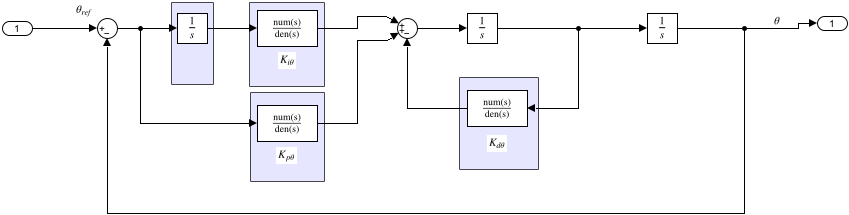
\includegraphics[width=0.8\linewidth]{Algebre_Diagrammes1.png}
    \caption{Étape 1}
    \end{figure}

    \begin{figure}[h!]
    \centering 
    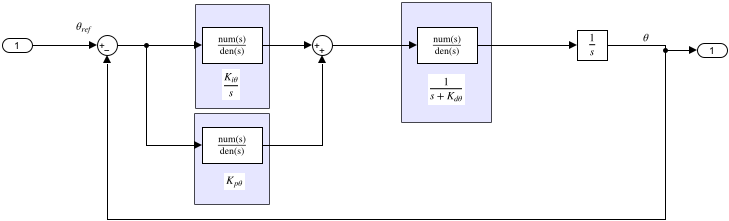
\includegraphics[width=0.8\linewidth]{Algebre_Diagrammes2.png}
    \caption{Étape 2}
    \end{figure}

    \begin{figure}[H]
    \centering 
    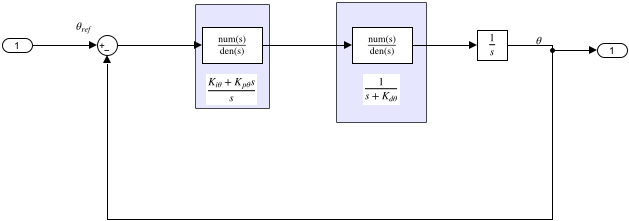
\includegraphics[width=0.8\linewidth]{Algebre_Diagrammes3.png}
    \caption{Étape 3}
    \end{figure}

    \begin{figure}[H]
    \centering 
    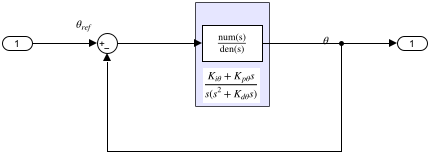
\includegraphics[width=0.8\linewidth]{Algebre_Diagrammes4.png}
    \caption{Étape 4}
    \end{figure}

    La forme finale du diagrame fonctionnel de $\theta$ est une boucle de rétroaction négative simple dont la fonction de transfert est: \newline

    \begin{center}
        \LARGE \text{$\frac{\Theta(s)}{\Theta_{ref}(s)}=\frac{\frac{K_{i\theta}+K_{p\theta}s}{s(s^2+K_{d\theta}s)}}{1+\frac{K_{i\theta}+K_{p\theta}s}{s(s^2+K_{d\theta}s)}}=\frac{K_{i\theta}+K_{p\theta}s}{s(s^2+K_{d\theta}s)+K_{i\theta}+K_{p\theta}s}$} 
    \end{center}

    \begin{center}
        $\boxed{\therefore \large \text{$\frac{\Theta(s)}{\Theta_{ref}(s)}=\frac{K_{i\theta}+K_{p\theta}s}{s^3+K_{d\theta}s^2+K_{p\theta}s+K_{i\theta}}$}}$
    \end{center}

    On voit qu'en remplaçant les valeurs de $K_{p\theta}$, $K_{i\theta}$ et $K_{d\theta}$ par leurs valeurs respectives de 39.5, 0.6 et 13.4, on obtient la même fonction de transfert que celle trouvée avec MATLAB: \newline
    \begin{center}
        \LARGE \text{$\frac{\Theta(s)}{\Theta_{ref}(s)}=\frac{39.5s+0.6}{s^3+13.4s^2+39.5s+0.6}$}
    \end{center}
    
    \newpage

    b) Tracer $\theta(t)$ et $\theta_{ref}(t)$ \newline
    Pour tracer les courbes de $\theta(t)$ et $\theta_{ref}(t)$, nous avons fait un diagramme fonctionnel identique à celui de la figure 2 de l'énoncé du devoir:

    \begin{figure}[H]
    \centering 
    \fbox{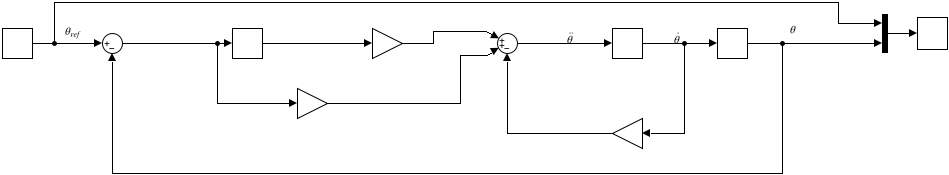
\includegraphics[width=0.8\linewidth]{Schema_Fonctionnel_angle.png}}
    \caption{Diagramme fonctionnel de l'angle $\theta$}
    \end{figure}
    Ensuite, nous avons écrit le script MATLAB suivant dans le fichier \text{script-devoir2.m}: \newline
    
    \lstinputlisting[language=Matlab,linerange={45-61},inputencoding=utf8/latin1]{script_devoir2.m} 
	\newpage
    En exécutant le code ci-dessus, on obtient le graphe suivant: \newline
    
    \begin{figure}[H]
    \centering 
    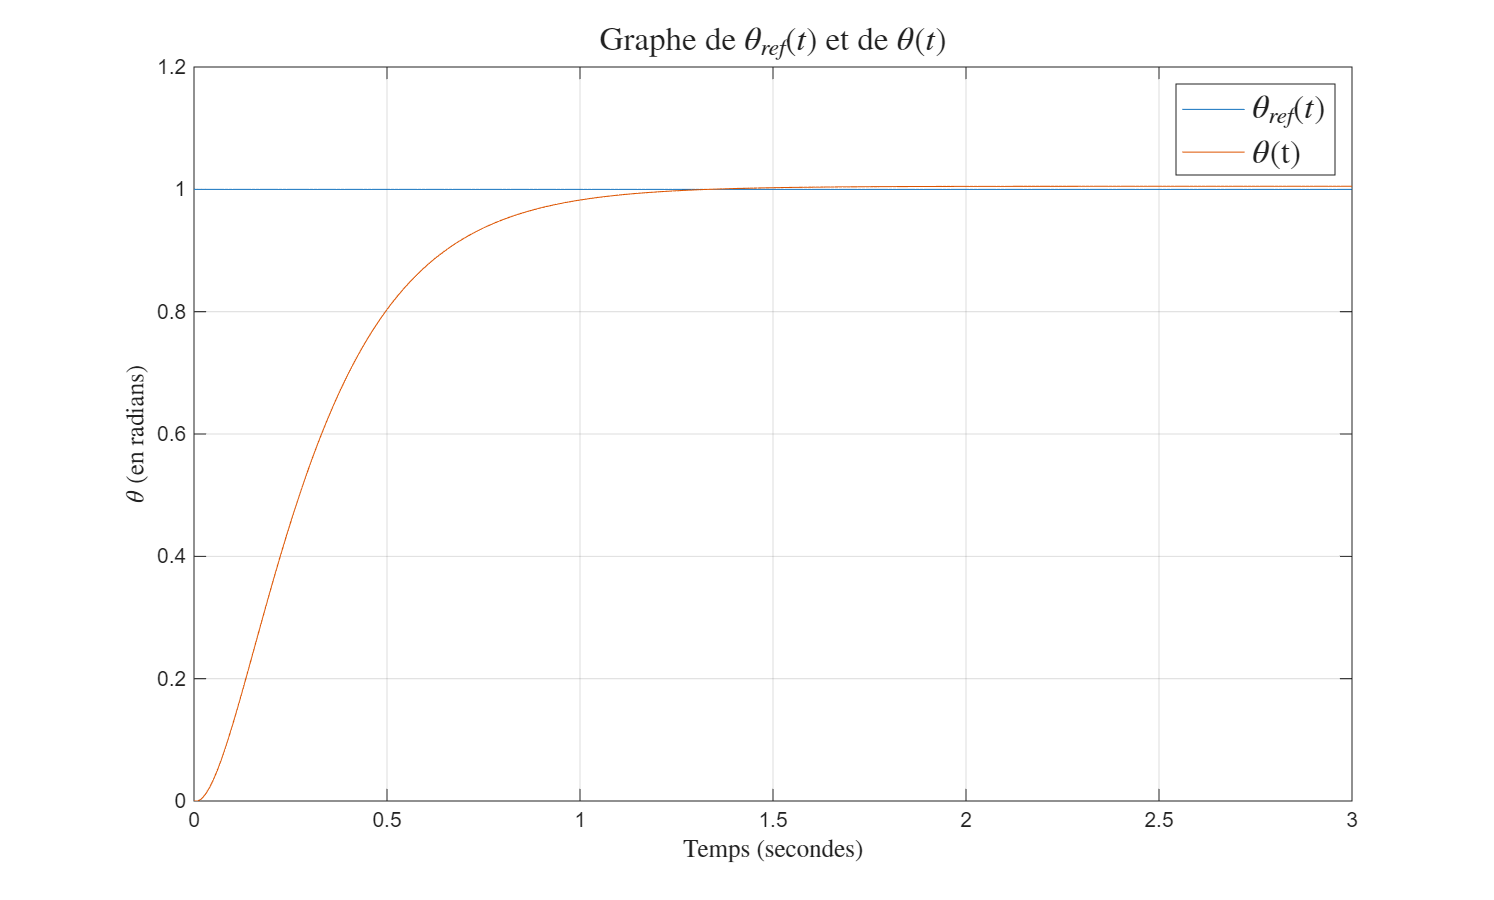
\includegraphics[width=0.8\linewidth]{Graphe_Q1_b).png}
    \caption{Graphe de $\theta(t)$ et $\theta_{ref}(t)$}
    \end{figure}

    La réponse $\theta(t)$ à l'entrée échelon unité $\theta_{ref}(t)$ a bel et bien le comportement attendu. On s'attendait à ce que le système soit stable en régime permanent car les pôles de la fonction de transfert sont tous du côté gauche du plan complexe. En utilisant la fonction "pole()" et en y mettant la fonction de transfert déclarée auparavant en argument, on obtient les valeurs  -9.0359, -4.3488 et -0.0153 qui sont toutes dans la partie gauche du plan complexe. Puisque l'entrée est un échelon unité et que le critère de stabilité est respecté (pôles), il est normal que la sortie se stabilise vers la forme de l'entrée lorsque le système entre en régime permanent, i.e. que la sortie $\theta(t)$ tende vers 1 lorsque t tend vers l'infini.
\newline 
    
    
    \section{Question 2: Contrôle de la position en x et y}
    a) Boucle en commande en y: calculer $\frac{Y(s)}{Y_{ref}(s)}$ \newline
    Il y a plusieurs approches possibles. On peut le trouver à l'aide de MATLAB et Simulink. D'abord, on effectue le diagramme fonctionnel de la commande en y dans Simulink (identique à celui de la figure 4 de l'énoncé): \newline

    \begin{figure}[H]
    \centering 
    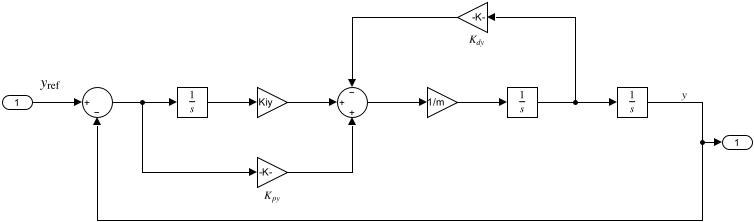
\includegraphics[width=0.8\linewidth]{Diagramme_Y.png}
    \caption{Diagramme fonctionnel de la commande en y}
    \end{figure}
    
    Ensuite, on fait exéctuer le script MATLAB suivant: \newline
    
     \lstinputlisting[language=Matlab,linerange={77-84},inputencoding=utf8/latin1]{script_devoir2.m}
     On obtient la fonction de transfert suivante: \newline
     \begin{center}
     \LARGE \text{$\frac{Y(s)}{Y_{ref}(s)}=\frac{75s+125}{s^3+15s^2+75s+125}$}
     \end{center}
     On peut aussi obtenir la fonction de transfert en faisant de l'algèbre des diagrammes avec le diagramme fonctionnel de la commande en y. \newline 
    \begin{figure}[H]
    \centering 
    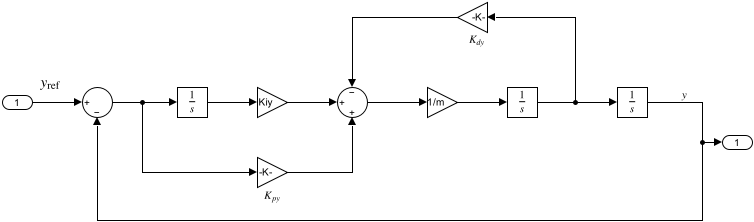
\includegraphics[width=0.8\linewidth]{Algebre_Y1.png}
    \caption{Étape 1}
    \end{figure}
    
    \begin{figure}[H]
    \centering 
    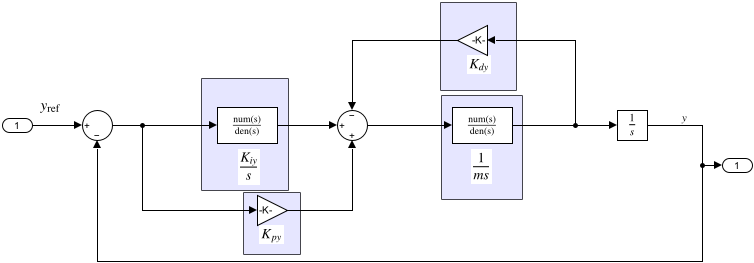
\includegraphics[width=0.8\linewidth]{Algebre_Y2.png}
    \caption{Étape 2}
    \end{figure}
    
    \begin{figure}[H]
    \centering 
    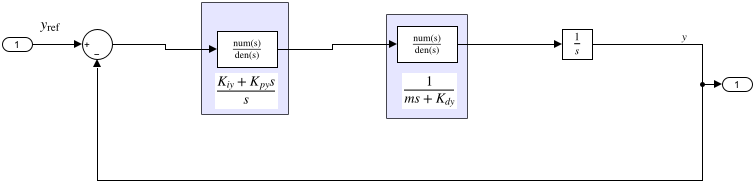
\includegraphics[width=0.8\linewidth]{Algebre_Y3.png}
    \caption{Étape 3}
    \end{figure}
    
    \begin{figure}[H]
    \centering 
    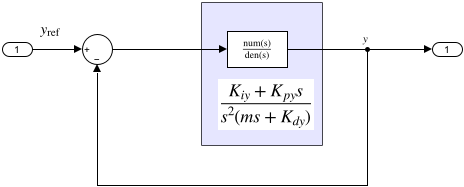
\includegraphics[width=0.8\linewidth]{Algebre_Y4.png}
    \caption{Étape 4}
    \end{figure}
    La forme à l'étape 4 ci-dessus est celle d'une simple boucle de rétroaction négative dont la fonction de transfert est: \newline
	\begin{center}	
	\LARGE \text{$\frac{Y(s)}{Y_{ref}(s)}=\frac{\frac{K_{iy}+K_{py}s}{s^2(ms+K_{dy})}}{1+\frac{K_{iy}+K_{py}s}{s^2(ms+K_{dy})}}=\frac{K_{iy}+K_{py}s}{s^2(ms+K_{dy})+K_{iy}+K_{py}s}$} \newline 
	\large \text{$\boxed{\therefore \frac{Y(s)}{Y_{ref}(s)}=\frac{K_{iy}+K_{py}s}{ms^3+K_{dy}s^2+K_{py}s+K_{iy}}}$}  
    \end{center}

	b) Boucle en commande en x: calculer $\frac{X(s)}{X_{ref}(s)}$
	
	Encore une fois, il existe plusieurs approches. On peut la calculer en utilisant MATLAB et Simulink. D'abord, on fait le diagramme fonctionnel suivant sur Simulink:
	\begin{figure}[H]
    \centering 
    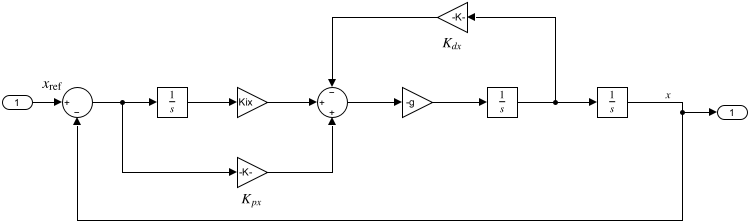
\includegraphics[width=0.8\linewidth]{Schema_X_Q2b.png}
    \caption{Diagramme fonctionnel de la commande en x} 
    \end{figure}
    On écrit le script suivant sur MATLAB:
     \lstinputlisting[language=Matlab,linerange={90-97},inputencoding=utf8/latin1]{script_devoir2.m} 
     Puis on obtient la fonction de transfert suivante: \newline
     \begin{center}
		\LARGE \text{$\frac{X(s)}{X_{ref}(s)}=\frac{4.316s+1.727}{s^3+3.6s^2+4.316s+1.727}$}     
     \end{center}
On peut aussi faire de l'algèbre des diagrammes pour obtenir la fonction de transfert, mais sous forme littérale (i.e. avec les variables $K_{px}$, $K_{ix}$, $K_{dx}$ laissées telles quelles):

	\begin{figure}[H]
    \centering 
    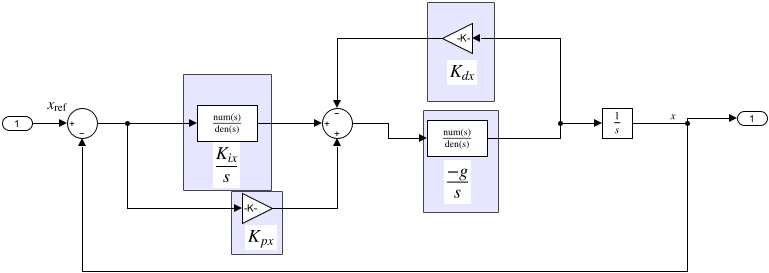
\includegraphics[width=0.8\linewidth]{Algebre_X1.png}
    \caption{Étape 1} 
    \end{figure}
    
    \begin{figure}[H]
    \centering 
    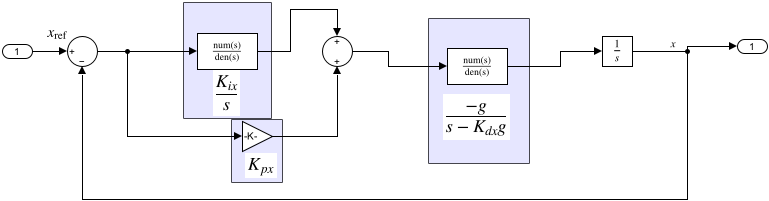
\includegraphics[width=0.8\linewidth]{Algebre_X2.png}
    \caption{Étape 2} 
    \end{figure}
    
    \begin{figure}[H]
    \centering 
    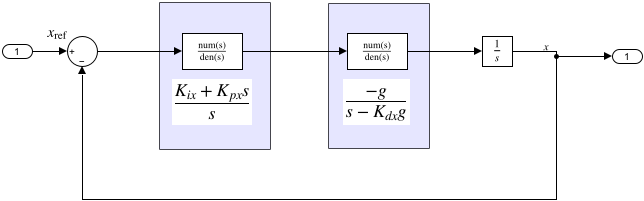
\includegraphics[width=0.8\linewidth]{Algebre_X3.png}
    \caption{Étape 3} 
    \end{figure}
    
    \begin{figure}[H]
    \centering 
    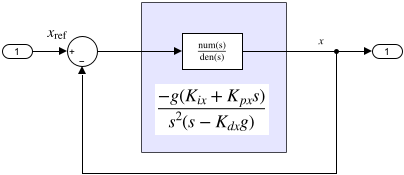
\includegraphics[width=0.8\linewidth]{Algebre_X4.png}
    \caption{Étape 4} 
    \end{figure}
Le diagramme ci-dessus correspond à la forme d'un système bouclé simple, en rétroaction négative, dont la fonction de transfert est la suivante: \newline

	\begin{center}
	\LARGE \text{$\frac{X(s)}{X_{ref}(s)}=\frac{\frac{-g(K_{ix}+K_{px}s)}{s^2(s-K_{dx}g)}}{1+\frac{-g(K_{ix}+K_{px}s)}{s^2(s-K_{dx}g)}}=\frac{-gK_{ix}-gK_{px}s}{s^3-gK_{dx}s^2-gK_{px}s-gK_{ix}}$} \newline 
	 \large \text{$\boxed{\therefore \frac{X(s)}{X_{ref}(s)}=\frac{-gK_{ix}-gK_{px}s}{s^3-gK_{dx}s^2-gK_{px}s-gK_{ix}}}$}
	\end{center}
En remplaçant $K_{px}$, $K_{ix}$, $K_{dx}$ et $g$ par leurs valeurs numériques respectives (i.e. respectivement -0.440, -0.176, -0.367 et 9.81), on retrouve la fonction de transfert trouvée sur MATLAB: \newline 
	\begin{center}
		\LARGE \text{$\frac{X(s)}{X_{ref}(s)}=\frac{-(9.81)(-0.176)-(9.81)(-0.440)s}{s^3-(9.81)(-0.367)s^2-(9.81)(-0.440)s-(9.81)(-0.176)}=\frac{1.727+4.316s}{s^3+3.6s^2+4.316s+1.727}$}
	\end{center}
	
c) Réponses indicielles $x(t)$ et $y(t)$ \newline \newline
On doit tracer les réponses indicielles $x(t)$ et $y(t)$ lorsque les entrées $x_{ref}(t)$ et $y_{ref}(t)$ sont respectivement des échelons unitaires. On effectue le diagramme fonctionnel ci-dessous sur Simulink: \newline

	\begin{figure}[H]
    \centering 
    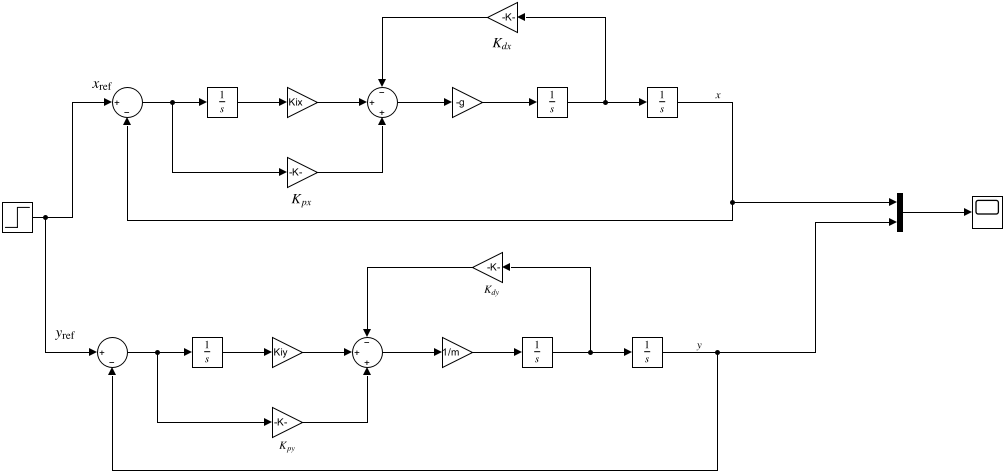
\includegraphics[width=0.8\linewidth]{Diagrammes_X_Y.png}
    \caption{Diagrammes fonctionnels des boucles en x et y} 
    \end{figure}
    
Ensuite, on exécute le script suivant sur MATLAB: \newline
     \lstinputlisting[language=Matlab,linerange={106-122},inputencoding=utf8/latin1]{script_devoir2.m}
     
On obtiens le graphe suivant:
    \begin{figure}[H]
    \centering
    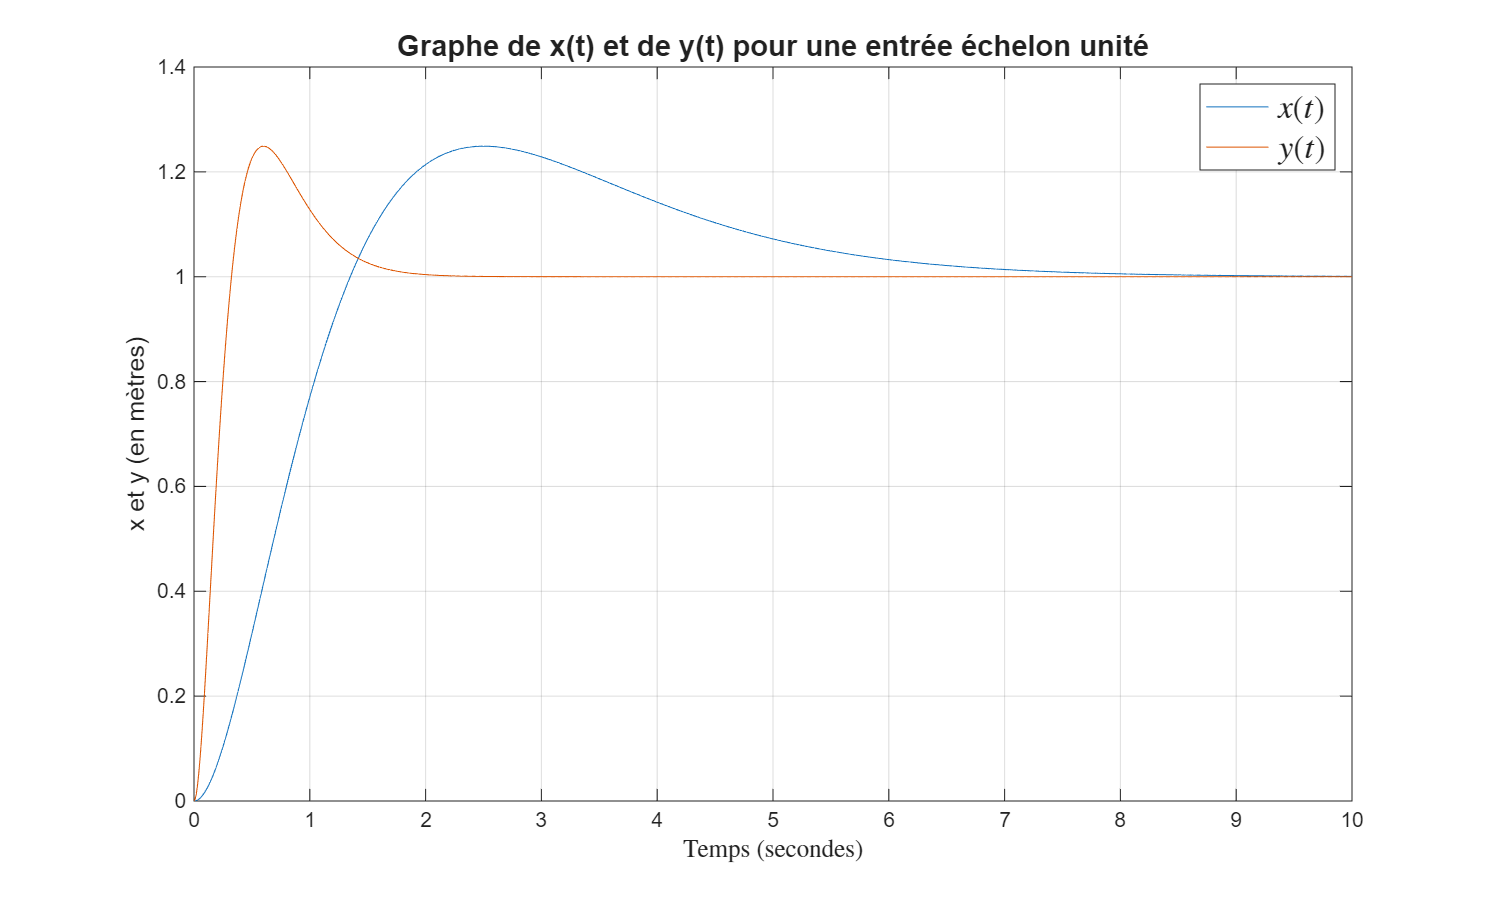
\includegraphics[width=0.8\linewidth]{Graphe_Q2_c.png}
    \caption{Graphe des positions x(t) et y(t) pour une entrée échelon unité} 
    \end{figure}
    
En utilisant la fonction "stepinfo()" de MATLAB (où les arguments des fonctions "linmod(...)" sont des fichiers Simulink), pour chaque boucle (en x et en y):
 \lstinputlisting[language=Matlab,linerange={77-85},inputencoding=utf8/latin1]{script_devoir2.m}
  \lstinputlisting[language=Matlab,linerange={91-99},inputencoding=utf8/latin1]{script_devoir2.m}
  on obtient les résultats suivants: \newline
  \begin{table}[H]
	\centering
	\resizebox{0.8\textwidth}{!}{
	\begin{tabular}{|c|c|c|}
	\hline
	Boucle & Dépassement (\%) & Temps de réponse à 2\% (secondes) \\
	\hline
	x & 25 & 6.58 \\
	\hline
	y & 25 & 1.58 \\
	\hline
	\end{tabular}}
	\caption{Dépassement et temps de réponse à 2\% pour les boucles en x et en y}
	\end{table} 
D'abord, on peut remarquer que les résultats du tableau 1 ci-dessus correspondent au graphe de la figure 18 i.e. le graphe des réponses indicielles $x(t)$ et $y(t)$. En effet, on peut constater que $y(t)$ se stabilise plus rapidement vers 1 que $x(t)$, ce qui concorde avec les résultats du tableau 1. On constate également que le dépassement est de 25\% pour les deux boucles. En effet, on peut voir dans le graphe de la figure 18 que les deux courbes $x(t)$ et $y(t)$ ont bel et bien la même valeur maximale, d'où la valeur de dépassement identique aux deux boucles. En somme, le régime transitoire de $y(t)$ est plus court que celui de $x(t)$. La réponse $y(t)$ atteint le même valeur maximale que la réponse $x(t)$, mais plus rapidement et elle décroit et se stabilise plus rapidement vers 1 (forme de l'entrée, qui est un échelon unité).
\end{document}